\section{Study 5: remote emotion detection}
\label{s:experiment1-study5}

%%%%%%%%%%%%%%%%%%%%%%%%%%%%%%%%%%%%%%%%%%%%%%%%%%%%%%%%%%%%%%%%%%%%%%%%%
\subsection{Introduction}
%%%%%%%%%%%%%%%%%%%%%%%%%%%%%%%%%%%%%%%%%%%%%%%%%%%%%%%%%%%%%%%%%%%%%%%%%

This study presents information regarding the use of machine learning to remotely detect the emotional state of subjects while they play a game. A set of features, including automatically detected facial cues and remote-estimated HR, are used to  A neural network is trained from

%This study presents information regarding the accuracy evaluation of a remote photoplethysmography (rPPG) technique in a gaming context. The technique was applied to estimate the HR of subjects behaving naturally in gaming sessions with induced boredom and stress. Previous work with experiments involving emotions and rPPG were performed under extremely controlled situations with few game-related stimuli. Subjects were not interacting with a complete digital game in any of the experiments, which hindered the accuracy evaluation of rPPG techniques within the context of games research, for instance. Authors commonly used images, videos or text as content to produce the emotional stimuli, in experimental sessions lasting from 20 seconds to 10 minutes.

%This study will describe my tests regarding the use of machine learning to detect the emotional state of subjects in my first experiment. The idea is to present this study as a planning for the second experiment. I will present the features used in the machine learning model, e.g. remote HR, eyebrow movement, etc, as a consequence of the previous studies.

%The focus will be on the features used and the accuracy achieved. I imagine a plausiable hypothesis for this study is "is the model able to detect emotions with an accuracy that is better than chance?". In the discussion, I will present how some features influence the results, e.g. facial features only versus HR only. I will not mention the idea of user-tailored versus group-tailored, because it will make things too complex to describe and argue about. My idea is to save that discussion for upcoming papers.

%%%%%%%%%%%%%%%%%%%%%%%%%%%%%%%%%%%%%%%%%%%%%%%%%%%%%%%%%%%%%%%%%%%%%%%%%
\subsection{Method and analysis}
\label{s:experiment1-study5-method}
%%%%%%%%%%%%%%%%%%%%%%%%%%%%%%%%%%%%%%%%%%%%%%%%%%%%%%%%%%%%%%%%%%%%%%%%%

%%%%%%%%%%%%%%%%%%%%%%%%%%%%%%%%%%%%%%%%%%%%%%%%%%%%%%%%%%%%%%%%
\subsubsection{Data pre-processing}

The pre-processing of video recordings involved extraction of the parts containing the interaction with the games and the discard of noisy frames. Firstly the periods where subjects were playing each one of the available games were extracted from the video recordings. It resulted in three videos per subject, denoted as $V_{s,i}$ where $s$ is the $s$-th subject and $i \in \{1, 2, 3\}$ represents the game.

\begin{figure}
\centering
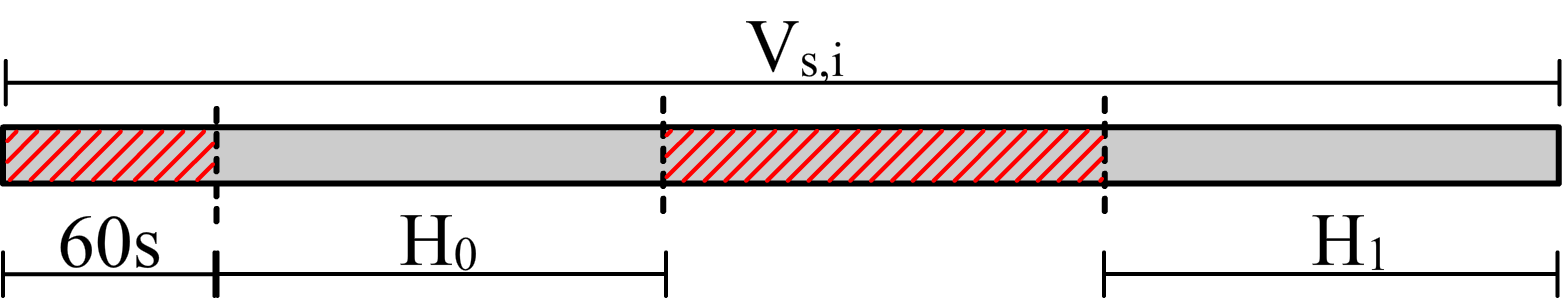
\includegraphics[width=0.9\textwidth]{figures/pre-processing}
\caption{Extraction of video segments $H_0$ and $H_1$ containing boring and stressful game interactions, respectively. Initial 60 seconds of any video $V_{s,i}$ are ignored and the remaining is divided into three pieces, from which the first and the last ones are selected. Stripes highlight discarded video segments.}
\label{fig:preprocessing}
\end{figure}

As previously mentioned, the games used as emotional elicitation material in the experiment induced variations of physiological signals on subjects, who perceived them as being boring at the beginning and stressful at the end. Since the aim of the present study is to test the potential of facial features to differentiate emotional states of boredom and stress, two video segments were extracted from each video $V_{s,i}$, named $H_0$ and $H_1$, whose subject's emotional state is assumed to be known and related to boredom and stress. In order to achieve that, the following extraction procedure was performed, illustrated in Figure \ref{fig:preprocessing}. Firstly the initial 60 seconds of any given video $V_{s,i}$ were ignored. The remaining of the video was then divided into three pieces, from which the first and the last were selected as $H_0$ and $H_1$, respectively.

The reason why the initial part of all game videos was discarded is because the first minute might not be ideal for a fair analysis. During the first minute of gameplay, subjects are less likely to be in their usual neutral emotional state. They are more likely to be stimulated by the excitement of the initial contact with a game soon to be played, which interferes with any feelings of boredom. Additionally subjects need basic experimentation with the game to learn how to play it and judge if it is boring or not. Such claim is supported by empirical analysis of the first minute of the video recordings that show repeated head and eye movements from and towards the keyboard/display. Consequently, the second minute and onward in the videos is more likely to portrait facial activity related to emotional reactions to the game instead of facial activity connected to gameplay learning. Regarding the division of the remaining part of the video into three segments, from which two were selected as $H_0$ and $H_1$, it followed the reasoning that the emotional state of subjects was unknown in the middle part of $V_{s,i}$. Based on self-reported emotional states, subjects reported the beginning part of the games as boring and the final part as stressful; additionally there are significant differences in the HR mean between the second and the last minute of gameplay in the games \parencite{bevilacqua2018changes}. As a consequence it is assumed that video segments $H_0$ and $H_1$ accurately portray interaction of subjects during boring and stressful periods of the games, respectively.

The pre-processing of the recordings resulted in 6 video segments per subjects: 3 segments $H_0$ (one per game) and 3 segments $H_1$ (one per game). A given game $i$ contains $N=20$ pairs of $H_0$ and $H_1$ video segments (20 segments $H_0$, one per subject, and 20 segments $H_1$, one per subject). When considering all subjects and games, there are $N=60$ pairs of $H_0$ and $H_1$ video segments (3 games $\times$ 20 subjects, resulting in 60 segments $H_0$ and 60 segments $H_1$). Subject 9 had problems playing the Platformer game, so segments $H_0$ and $H_1$ from subject 9 in the Platformer game were discarded. Consequentially the Platformer game contains $N=19$ pairs of $H_0$ and $H_1$ video segments; regarding all games and subjects, there are $N=59$ pairs of $H_0$ and $H_1$ video segments.

\subsubsection{Classification features}
%%%%%%%%%%%%%%%%%%%%%%%%%%%%%%%%%%%%%%%%%%%%%%%%%%%%%%%%%%%%%%%%%%%%%%%%%

The classification efficiency of a machine learning model is related to the number of features able to accurately discriminate the elements being classified. The use of more features does not necessarely produce a better model. Some features might not accurately contribute to the classification, which leads to degradation of results if they are included.

Features and their classification potential are highly dependent on the type of data being used. In the present study, the set of features used for classification was extracted and selected based on previous reports of the potential of said features to differentiate emotional states in games. In total 8 features, denoted $F_1$ to $F_8$, are available for use: $F_1$ to $F_7$ are related to facial activity and $F_8$ to $F_11$ are related to HR activity, including remote estimations (rPPG). Table \ref{table:study5-features-list} presents a description of all features.

\begin{table*}
    \centering
    \caption{Description of features used for classification}
    \label{table:study5-features-list}
    \begin{tabular}[l]{@{}clp{6.5cm}}
        \hline
            \textbf{Notation} & \textbf{Name} & \textbf{Description} \\
        \hline
            $F_1$ & Mouth outer & Monitor the zygomatic muscle.  \\
            $F_2$ & Mouth corner & Monitor the zygomatic muscle. \\
            $F_3$ & Eye area & Monitor the orbicularis oculi muscle. \\
            $F_4$ & Eyebrow activity & Monitor the corrugator muscle.  \\
            $F_5$ & Face area & Monitor facial movement to and away from the camera  \\
            $F_6$ & Face motion & Describe the total distance the head has moved in any direction in a short period of time.  \\
            $F_7$ & Facial COM & Describe the overall movement of all facial landmarks. \\
            $F_8$ & Remote HR & HR estimated using the rPPG technique proposed by \textcite{poh2011advancements}.  \\
            $F_9$ & Ground HR & HR estimated   \\
            $F_10$ & Normalized remote HR & HR estimated   \\
            $F_11$ & Normalized ground HR & HR estimated   \\
        \hline
    \end{tabular}
\end{table*}

Features $F_1$ to $F_7$ are based on automatically detected facial landmarks related to facial elements that express a connection with emotional states. As previsouly mentioned in Chapter \ref{ch:literature-face}, there is evidence of more frequent corrugator activity when positive game events occur \parencite{hazlett2006measuring} and increased activity of zygomatic muscle associated with self-reported positive emotions \parencite{tijs2008dynamic}. Positive and rewarding game events are also connected to increase in zygomatic and orbicularis oculi activity \parencite{ravaja20051}. Detection of stress is also related to blinking rate \parencite{giannakakis2017stress,dinges2005optical}, lip movement \parencite{dinges2005optical} and lips deformation \parencite{metaxas2004image,giannakakis2017stress}, mouth activity \parencite{liao2005decision}, and head movement/velocity \parencite{giannakakis2017stress}.

Feature $F_8$ is based on remote estimations of HR performed using the rPPG technique proposed by \textcite{poh2011advancements}. As previously mentioned in Chapter \ref{ch:literature-physiological}, HR and its derivatives, such as HRV, have been used as reliable sources of information in different emotion estimation methods \parencite{kukolja2014comparative}. Reports in the literature show the use of HR and derivates for continuous arousal monitoring \parencite{grundlehner2009design}, measurement of confusion \parencite{xiao2015towards}, triangulation of phychophysiological emotional reactions to digital media stimuli \parencite{nogueira2015annotation}, detection of mental and physical stress \parencite{vandeput2009heart,garde2002effects}, and measurement of frustration \parencite{rodriguez2015vr}.

\subsubsection{Features extraction and calculation}
%%%%%%%%%%%%%%%%%%%%%%%%%%%%%%%%%%%%%%%%%%%%%%%%%%%%%%%%%%%%%%%%%%%%%%%%%

The process of extracting and calculating features is performed using a moving window applied on the videos of all subjects. The moving window has a size of 15 seconds and a step of 1 second (93.33\% overlap). For each window in the video, computer vision techniques are applied to all frames within that window to detect facial landmarks and to collect information regarding pixel values, e.g. mean value of pixels in the blue channel. The detected landmarks are used to calculate the features related to facial activity, while pixel values are used to estimate the HR.

Features $F_1$ to $F_7$, which represent facial activity, are mostly calculated using the Euclidian distance of automatically detected facial landmarks for each frame. A detailed description of the process is presented in Section \ref{s:study4} (page \pageref{s:study4}). Feature $F_8$, which represent HR activity, is calculated based on remote estimations of HR. A detailed description of the process is presented in Section \ref{s:study3} (page \pageref{s:study3}).

Even though all frames within the window are analyzed, only a single, final value is assigned to each feature per window. For features $F_1$ to $F_7$, the final value of a given feature is calculated by aggregating the values of all frames within the window of that given feature using mean, standard deviation or sum. From now on, $F_i^\mu$, $F_i^\sigma$, and $F_i^\Sigma$ will be used to denote feature $F_i$ whose values in a window were aggregated using mean, standard deviation and sum, respectively. Feature $F_8$ does not require any aggregation of values since all frames within the window are used to produce a single value, i.e. the estimation of the mean HR in that window.

\subsubsection{Training and evaluation of an emotion classifier}
\label{s:experiment1-study5-training-evaluation}
%%%%%%%%%%%%%%%%%%%%%%%%%%%%%%%%%%%%%%%%%%%%%%%%%%%%%%%%%%%%%%%%%%%%%%%%%

The classification procedure uses the previously mentioned feature set and a neural network trained to identify two emotional states: boredom and stress. Both the training and evaluation of the neural network are performed on a user tailored fashion: data from a given subject $S_i$ is used to train and evaluate the emotion classification of that given subject $S_i$. Figure \ref{fig:study5-training-evaluation} illustrates the process.

\begin{figure}[ht]
\centering
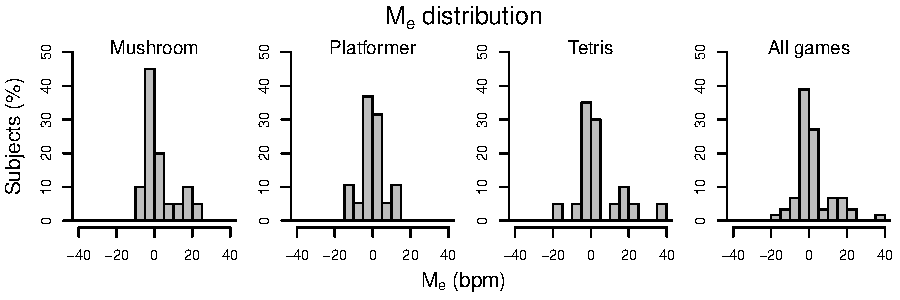
\includegraphics[width=1.0\textwidth]{figures/hist-me.pdf}
\caption{Something about training and evaluation}
\label{fig:study5-training-evaluation}
\end{figure}

Leave One Session Out Cross Validation (LOSOCV) is used to evaluate each trained user-tailored model, as illustrated in Figure \ref{fig:study5-training-evaluation}(a). In LOSOCV, data from one session instance is left out and a model is constructed on data from all other session instances. In the present study, a given subject $S_i$ played 3 calibration games, so data from one calibration game is left out and a model is trained on the data of the other two calibration games for that subject $S_i$. This is repeated for all three calibration games of that subject $S_i$. Consequentially the use of LOSOCV will produce 3 models per subject, resulting in 3 measurements of classificaiton accuracy per subject (one for each model being evaluated). The final classification accuracy for a given subject $S_i$, named $A_i$, is the mean of those three values that were obtained from the iterations in the LOSOCV. In other words, each subject contributes a single classification accuracy value $A_i$, which is calculated based on the mean classification accuracy of his/her three models in the LOSOCV iterations.

In the training process of each model, which is performed 3 times per user as illustrated in Figure \ref{fig:study5-training-evaluation}(b), the hyper-parameters of each neural network, e.g. number of neurons, is optimized using random search \parencite{bergstra2012random}. A 10-fold cross validation method repeated 3 times is applied, so the dataset is split into 10-subsets and each of those subset is held out while the model is trained on all others. The process is repeated 3 times and the final metric for the model is the mean from the number of repeats. Area under the ROC curve (AUC) is used as a metric to select the best model in the 10-fold cross validation.

According to previous analysis, subjects perceived the games as being boring at the beginning and stressful at the end. As a consequence, it is assumed that subject's emotional state in $H_0$ and $H_1$ is boredom and stress, respectively. Based on that assumption, training and evaluation data obtained from video segments in $H_0$ and $H_1$ were labeld as boredom and stress, respectively.

%, which finds models as good or beter then ones configured by a pure grid search

%Describe how the model was trained, which includes how the calibration games were grouped, e.g. two for training, one for testing. Explain that neural networks were used because they are widely mentioned in the literature.

%%%%%%%%%%%%%%%%%%%%%%%%%%%%%%%%%%%%%%%%%%%%%%%%%%%%%%%%%%%%%%%%%%%%%%%%
\subsubsection{Analysis}
\label{s:experiment1-study5-analysis}
%%%%%%%%%%%%%%%%%%%%%%%%%%%%%%%%%%%%%%%%%%%%%%%%%%%%%%%%%%%%%%%%%%%%%%%%%

In order to test the effectiveness of the neural network in classifying samples as either boredom or stress, all trained neural networks were evaluated in conjunction. As described in the previous section, each subject's model was evaluated using LOSOCV, which produced a classification accuracy $A_i$ for any given subject $S_i$. The minimum, maximum and mean value of $A_i$ was calculated as a metric for accuracy. In order to provide better contextualization of the classification results, the same process was also applied to other three metrics obtained during the LOSOCV evaluation: precision, recall and F1 score.

Aiming to better understand the contribution of each feature for the classification process, the training/evaluation process mentioned early was also performed using different feature sets. Each of those different feature sets was evaluated in an independent test, denoted $T_i$. Table \ref{table:study5-different-feature-sets} shows the tests $T_i$ and the corresponding feature sets used in the process.

\begin{table*}
    \centering
    \caption{Tests and their respective feature sets}
    \label{table:study5-different-feature-sets}
    \begin{tabular}[l]{@{}cp{9cm}}
        \hline
            \textbf{Name} & \textbf{Feature set} \\
        \hline
            \texttt{MULTI\_R} & 5278d175-71e752ce \\ % HR_poh2011, mean_face_activity_mouth_corner, mean_face_activity_mouth_outer, mean_face_area, std_face_activity_eyebrow, std_face_eye_area, std_face_motion_instability
            \texttt{MULTI\_G} &  5278d175-9fa716ee  \\ % mean_HR_ground, mean_face_activity_mouth_corner, mean_face_activity_mouth_outer, mean_face_area, std_face_activity_eyebrow, std_face_eye_area, std_face_motion_instability
            \texttt{FACE} &  5278d175-826512b2  \\ % mean_face_activity_mouth_corner, mean_face_activity_mouth_outer, mean_face_area, std_face_activity_eyebrow, std_face_eye_area, std_face_motion_instability
            \texttt{HR\_R} &  5278d175-97a38001  \\ % HR_poh2011
            \texttt{HR\_G} &  5278d175-ad2580a5 \\ % mean_HR_ground
        \hline
    \end{tabular}
\end{table*}

\todo[inline]{Better describe each test and their features.}

%As previously mentioned, both training and evaluation data for each subject were labeled as either boredom or stress according to the assumed emotional state during the interaction with the games. According to previous analysis, the value of the classification features during boring periods of the games are expected to be different than those during stressful periods.

Subjects perceived the games as boring and stressful, so such difference should make a trained neural network capable of properly classifying evaluation samples as either boredom or stress. Additionally the use of a multifactorial approach, where facial analysis and HR information are used in combination instead of either one alone, is expected to produce better classification results \parencite{zacharatos2014automatic}. Based on those expectations, the following hypotheses are stated:

\begin{itemize}
  \item[] \textit{$u_1$: a user-tailored neural network trained on data samples from two calibration games of a given subject $S_i$ is able to classify samples from a third calibration game of that same subject $S_i$ with an accuracy greater than chance-level rate (random guessing);}
  \item[] \textit{$u_2$: a user-tailored neural network using a multifactorial feature set, i.e. facial and HR features, performs with greater accuracy than a user-tailored neural network using facial features only;}
  \item[] \textit{$u_3$: a user-tailored neural network using a multifactorial feature set, i.e. facial and HR features, performs with greater accuracy than a user-tailored neural network using HR features only.}
\end{itemize}

Hypothesis $u_1$ was tested by checking if the mean value of the classification accuracy, i.e. calculated from all $A_i$ values, is greater than 0.5. In such case it is assumed that an accuracy rate of 0.5 (50\%) is the theoretical probabilistic chance level achieved by totally random classification performed by a classifier evaluated on an infinite number of data samples. Hypotheses $u_2$ and $u_3$ were tested by performing a Wilcoxon Signed Ranks test on all $A_i$ values of the two competing models.

\todo[inline]{Say that wilcoxon test was performed on all metrics (3 per subject), so N=57, not on their means.}

%%%%%%%%%%%%%%%%%%%%%%%%%%%%%%%%%%%%%%%%%%%%%%%%%%%%%%%%%%%%%%%%%%%%%%%%%
\subsection{Results}
%%%%%%%%%%%%%%%%%%%%%%%%%%%%%%%%%%%%%%%%%%%%%%%%%%%%%%%%%%%%%%%%%%%%%%%%%

Table \ref{table:study5-result-metrics-mean} presents the mean values of the resulting classification metrics for accuracy, precision, recall and F1 score, calculated and analyzed according to the procedures described in Section \ref{s:experiment1-study5-method}. Regarding the accuracy metric, the highest mean value achieved was 62.3\% in test \texttt{MULTI\_G}, whose model used a combination of facial and HR features. The HR feature in that case was calculated from the physical sensor, not remotely estimated. The second and third highest accuracy rates were 60.8\% in test \texttt{HR\_G} (HR from physical sensor only) and 60.4\% in test \texttt{MULTI\_R} (facial and remotely-estimared HR features), respectively. The highest values achieved for precision, recall and F1 score were 65.6\%, 62.4\%, and 58.1\%, respectively, all in test \texttt{HR\_G}.

\begin{table*}
    \centering
    \caption{Mean values of resulting classification metrics}
    \label{table:study5-result-metrics-mean}
    \begin{tabular}[l]{@{}ccccc}
        \hline
            \textbf{Test} & \textbf{Accuracy} & \textbf{Precision} & \textbf{Recall} & \textbf{F1}\\
        \hline
            \texttt{MULTI\_R} & 0.604 & 0.612 & 0.599 & 0.521 \\ % 5278d175-71e752ce
            \texttt{MULTI\_G} & \textbf{0.623} & 0.583 & 0.607 & 0.514 \\ % 5278d175-9fa716ee
            \texttt{FACE} & 0.594 & 0.601 & 0.585 & 0.507 \\ % 5278d175-826512b2
            \texttt{HR\_R} & 0.547 & 0.541 & 0.545 & 0.497 \\ % 5278d175-97a38001
            \texttt{HR\_G} & 0.608 & \textbf{0.656} & \textbf{0.624} & \textbf{0.581} \\ % 5278d175-ad2580a5
        \hline
    \end{tabular}
\end{table*}

Table \ref{table:study5-result-metrics-minmax} presents a discrimination of the minumum and maximum values for the resulting classification metrics. At least one subject in test \texttt{MULTI\_G} has been classified with an accuracy of 98\%, the highest value for that metric in all tests. The worst accuracy value was 19\% for at least one subject in test \texttt{MULTI\_R}. Regarding precision, the highest value was 97\% in test \texttt{MULTI\_G}. In all tests but \texttt{HR\_G}, at least one subject has been classified with zero precision (all samples were classified wrongly). Regarding precision, the highest and lowest values were 98\% and 12\% in tests \texttt{MULTI\_G} and \texttt{FACE}, respectively. Finally regarding F1 score, the highest value was 98\% for at least one subject in test \texttt{MULTI\_G}. All tests presented zero as the lowest F1 score.

\begin{table}[!htbp]
  \centering
  \caption{Minimum and maximum values of resulting classification metrics}
  \label{table:study5-result-metrics-minmax}
  \begin{tabular}{ccccccccc}
    \hline
      \textbf{Test} & \multicolumn{2}{c}{\textbf{Accuracy}} & \multicolumn{2}{c}{\textbf{Precision}} & \multicolumn{2}{c}{\textbf{Recall}} & \multicolumn{2}{c}{\textbf{F1}} \\
      {} & min & max & min & max & min & max & min & max \\
    \hline
      \texttt{MULTI\_R}  & 0.19 & 0.91 & 0.00 & 0.95 & 0.19 & 0.87 & 0.00 & 0.91 \\ % 5278d175-71e752ce
      \texttt{MULTI\_G}  & 0.25 & \textbf{0.98} & 0.00 & \textbf{0.97} & 0.13 & \textbf{0.98} & 0.00 & \textbf{0.98} \\ % 5278d175-9fa716ee
      \texttt{FACE}  & 0.26 & 0.90 & 0.00 & 0.95 & 0.12 & 0.90 & 0.00 & 0.89 \\ % 5278d175-826512b2
      \texttt{HR\_R}  & 0.36 & 0.72 & 0.00 & 0.79 & 0.18 & 0.77 & 0.00 & 0.67 \\ % 5278d175-97a38001
      \texttt{HR\_G}  & 0.38 & 0.82 & 0.26 & 0.85 & 0.23 & 0.87 & 0.00 & 0.81 \\ % 5278d175-ad2580a5
    \hline
  \end{tabular}
\end{table}

% data_multi_r and data_hr_r: p = 0.04488, Zstat = -2.0058, effect = 0.2657
% data_multi_r and data_face: p = 0.26797, Zstat = -1.1077, effect = 0.1467

Finally there are indications that a multifactorial model, which uses a combination of facial and HR features, performs with greater accuracy than a model using either facial or HR features. A Wilcoxon Signed Ranks test indicated that the accuracy was greater for a multifactorial model using facial and remotely estimated HR features, i.e. \texttt{MULTI\_R}, than for a model using only remotely estimated HR, i.e. \texttt{HR\_R}, $Z=-2.00$, $p=0.044$, $r=0.26$. However there are no indications that the accuracy of such multifactorial model, i.e. \texttt{MULTI\_R}, was statistically significantly greater than the accuracy of a model using only facil features, i.e. \texttt{FACE}, $Z=-1.10$, $p=0.267$, $r=0.14$.

%%%%%%%%%%%%%%%%%%%%%%%%%%%%%%%%%%%%%%%%%%%%%%%%%%%%%%%%%%%%%%%%%%%%%%%%%
\subsection{Discussion}
%%%%%%%%%%%%%%%%%%%%%%%%%%%%%%%%%%%%%%%%%%%%%%%%%%%%%%%%%%%%%%%%%%%%%%%%%

% data_multi_g and data_face: p = 0.03343, Zstat = -2.1269, effect = 0.2817
% data_multi_g and data_hr_g: p = 0.27802, Zstat = -1.0848, effect = 0.1437

% data_multi_g and data_multi_r: p = 0.07836, Zstat = -1.7603, effect = 0.2332

The results obtained indicate that the use of a user-tailored model to remotely estimate the emotional state of players from videos of gaming sessions is feasible. The previuly mentioned hypothesis $u_1$ states that a user-tailored neural network trained on data samples from two calibration games of a given subject $S_i$ is able to classify samples from a third calibration game of that same subject $S_i$ with an accuracy greater than chance-level rate (random guessing). Such model was tested in two configurations: \texttt{MULTI\_R} and \texttt{MULTI\_G}. Model \texttt{MULTI\_R}, which uses a multifactorial feature set composed of facial and remotely estimated HR information, presented a mean classification accuracy of 60.4\%. Such reported accuracy is greater than 50\%, the theoretical probabilistic chance level, which confirms hypothesis $u_1$. Model \texttt{MULTI\_G}, which also uses a multifactorial feature set but differs in the acquisition of HR data, i.e. physical sensor instead of remote estimation, presented a mean classification accuracy of 62.3\%. Such reported accuracy is also greater than the theoretical probabilistic chance level. The slightly greater classification accuracy of model \texttt{MULTI\_G} compared to \texttt{MULTI\_R} suggests that more precise rPPG estimations of the HR could improve the overall classification accuracy of model \texttt{MULTI\_R}. A Wilcoxon Signed Ranks test, however, has no statistically significant indication that the accuracy was greater for \texttt{MULTI\_G} than for \texttt{MULTI\_R}, $Z=-1.76$, $p=0.078$, $r=0.23$. Despite not being statistically signiciant, the $p$ value and Cohen's classification of $r=0.23$ as a small effect suggest a trend towards that reasoning.

Hypothesis $u_2$ states that a user-tailored neural network using a multifactorial feature set performs with greater accuracy than a user-tailored neural network using facial features only. The Wilcoxon Signed Ranks test mentioned in the previous section presented no statistically significant indications that the classification accuracy of \texttt{MULTI\_R} is greater than \texttt{FACE}. Such results refute hypothesis $u_2$ and suggest that a set of facial features, e.g. eyebrow and mouth analysis, has a greater potential to differentiate emotional states in a classifier, particuarly better than a classifier based on rPPG-estimated HR alone, in the context of this experiment.

Regarding hypothesis $u_3$, which states that a user-tailored neural network using a multifactorial feature set performs with greater accuracy than a user-tailored neural network using HR features only. The Wilcoxon Signed Ranks test mentioned in the previous section presented statistically significant indications that the classification accuracy of \texttt{MULTI\_R} is greater than \texttt{HR\_R}. It supports the claim of hypothesis $u_3$, confirming that a multifactorial model performs better than one based solely on remotely estimated HR data. The lower classification potential of remotely estimated HR, however, could be attributed to errors in the rPPG estimation process caused by noise, e.g. natural movement of subjects (see Section \ref{s:study3}, on page \pageref{s:study3}, for more information). As a consequence, a more precise HR estimation used in a multifactorial model allegedly contributes to produce a better classifier. A Wilcoxon Signed Ranks test confirms with statistical significance that the classification accuracy of \texttt{MULTI\_G} is greater than the accuracy of \texttt{FACE}, $Z=-2.12$, $p=0.033$, $r=0.28$. It supports the previously mentioned idea that a precise HR estimation (from a physical sensor in the case of \texttt{MULTI\_G}) combined with facial information is a better classifier than one using facial information alone, i.e. model \texttt{FACE}. Finally a Wilcoxon Signed Ranks test does not indicate that the accuracy of \texttt{MULTI\_G} is greater than \texttt{HR\_G}, $Z=-1.08$, $p=0.278$, $r=0.14$. Consequentially it seems that precise estimations of HR is important, but HR or facial information used separatedely are likely to be less important for classification then a joint, multifactorial use of them in the emotion classification process.

%The overarching hypothesis states that the mean value of features in $H_0$ is different than the mean value in $H_1$. The overarching hypothesis is composed of 7 sub-hypotheses. i.e. $u_i$, one for each feature $F_i$, where $u_i$ states that the true difference in means between the value of a given feature $F_i$ in $H_0$ and $H_1$, is greater than zero. The majority of the calculated facial features, i.e. mouth outer ($F_1$), mouth corner ($F_2$), eye area ($F_3$), eyebrow activity ($F_4$), and face area ($F_5$), presented statistically significant differences in their mean values when compared between two distinct parts of the games, i.e. $H_0$ and $H_1$. As previously mentioned, subjects perceived the first part of the games, i.e. $H_0$, as being boring and the second part, i.e. $H_1$, as being stressful. Results support the claim of sub-hypotheses $u_1$ to $u_5$, which indicate that facial features $F_1$ to $F_5$ can be differentiated between periods $H_0$ and $H_1$ and consequentially have the potential to unobtrusively differentiate emotional states of boredom and stress of players in gaming sessions. Results refute sub-hypotheses $u_6$ and $u_7$, since features $F_6$ and $F_7$ lack statistical significance to be differentiated between periods $H_0$ and $H_1$.





%%%%%%%%%%%%%%%%%%%%%%%%%%%%%%%%%%%%%%%%%%%%%%%%%%%%%%%%%%%%%%%%%%%%%%%%%
\subsection{Conclusions}
%%%%%%%%%%%%%%%%%%%%%%%%%%%%%%%%%%%%%%%%%%%%%%%%%%%%%%%%%%%%%%%%%%%%%%%%%


%\section{Definition of inputs for the user-tailored model}
%\label{sec:closing-definition-inputs}

%The literature review presented in chapters \ref{ch:literature-physiological}, \ref{ch:literature-face} and \ref{ch:literature-multifactorial} indicates that a model based on several user signals, which is a multifactorial analysis, is more efficient for emotion detection. The mentioned chapters also highlight which of those signals can be remotely acquired within the context of this research via computer vision techniques.

%\begin{figure}[h]
%    \centering
%    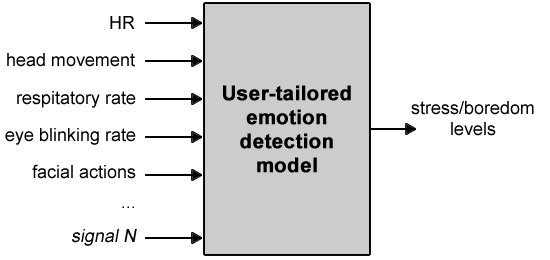
\includegraphics[width=0.6\textwidth]{figures/model-inputs-set.png}
%    \caption{Overall structure of the user-tailored emotion detection model regarding input (user signals) and output (stress/boredom levels).}
%    \label{fig:model-inputs-set}
%\end{figure}

%The user-tailored model proposed for this research might have $N$ input signals, varying from physiological ones, e.g. HR, to non-physiological ones, e.g. facial actions and head movements. Figure \ref{fig:model-inputs-set} illustrates the overall structure of the model. In order to be used in the model, an input signal needs to be supported by previous work regarding emotion detection, as well as be validated within the process of the proposed game-based calibration phase. Time and scope constraints limit the amount of input signals that can be implemented, evaluated and used in this research. As a consequence, a study will be conducted to investigate, validate and initially implement two of those signals into the proposed model: HR and facial activity (which includes head movement, lips activity, etc).

%The techniques and works presented in chapter \ref{ch:literature-face}, which relate to face detection and emotion estimation, suggest that facial analysis is an important component of a multifactorial emotion detection model. Empirical analysis of the data from the first experiment also suggest that individualities regarding facial activities do exist and could be used to estimate emotional states on a user-tailored basis \parencite{bevilacqua2016variations}. As described in section \ref{ch:literature-face-emotion-detection}, facial actions, head movement, lips/eye/mouth activity and distance measurements of detected facial landmarks are viable and proven sources of information for emotion detection.

%Regarding physiological signals, results indicate that the average HR mean for players during the last minute of gameplay is greater than the average HR mean during the second minute of gameplay (chapter \ref{ch:experiment1}, section \ref{s:study3}). The findings are aligned with and reinforce previous research that indicates higher HR mean during stressful situations in a gaming context. The findings also suggest that changes in the HR during gaming sessions is a promising indicator of stress.

%The study will involve the definition of how those two signals will be used as inputs for the model. Facial actions, for instance, will probably be detected and measured by the euclidian distance of the facial landmarks. A vector containing the distances will be evaluated as the input for the model. Regarding the HR, its mean and standard deviation during a particular analysis window will be evaluated as input for the model. A software for the detection of those two signals will be created and used to analyse the video recordings of the first experiment (chapter \ref{ch:experiment1}). The inclusion or exclusion of a component of a signal, e.g. variations of the distances of the lips landmark points, will be based on the accuracy to detect them and the frequency they appear in boring and stressful part of the calibration games.

%\section{Investigation of machine learning techniques}
%\label{closing:investigation-machine-learning}

%The majority of the previous work found in the literature mention the use of machine learning techniques to model user signals into emotional states. Different models and accuracy results are mentioned, which depend on several particularities of the approach used by the authors. A machine learning model will also be used by this research as a user-tailored emotion detection model.

%\begin{figure}[h]
%    \centering
%    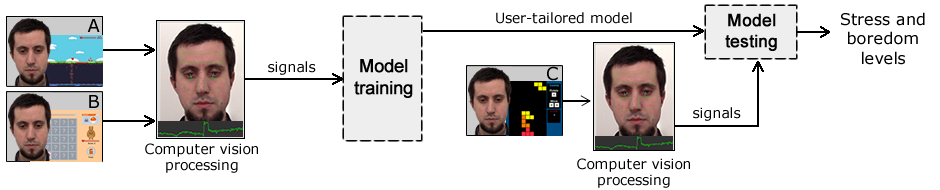
\includegraphics[width=\textwidth]{figures/machine-learning-investigation.png}
%    \caption{Iteration of a 3 fold cross validation performed on the video of a gaming sessions with 3 games, i.e. A, B and C. The videos of two calibration games, e.g. A and B, are used to train the machine learning model, while the video of the third calibration game, e.g. C, is used to test the model.}
%    \label{fig:machine-learning-investigation}
%\end{figure}

%A systematic study and accuracy evaluation will be performed to select the proper machine learning technique to be used in the model. The evaluation process will be conducted on each one of the selected (and competing) machine learning techniques using the video recordings of experiment 1. The evaluation is based on a 3 fold cross validation process, illustrated in Figure \ref{fig:machine-learning-investigation}. Initially the input signals for the emotion detection model (defined in the previous task, section \ref{sec:closing-definition-inputs}) will be extracted from two, e.g. A and B, of the three games played by a user and used to train the emotion detection model. The thrid game, e.g. C, that was left out of the training will be used as a testing set: user signals will be extracted from the video of that game and fed into the trained emotion detection model, which will output the predicted emotional state of the user. The 3 fold cross validation process is repeated three times, each one of them leaving out of the training phase a different game, i.e. A and B are used for training and C is used for testing, A and C are used for training and B for testing, and finally B and C are used for training and A for testing.

%\begin{figure}[h]
%    \centering
%    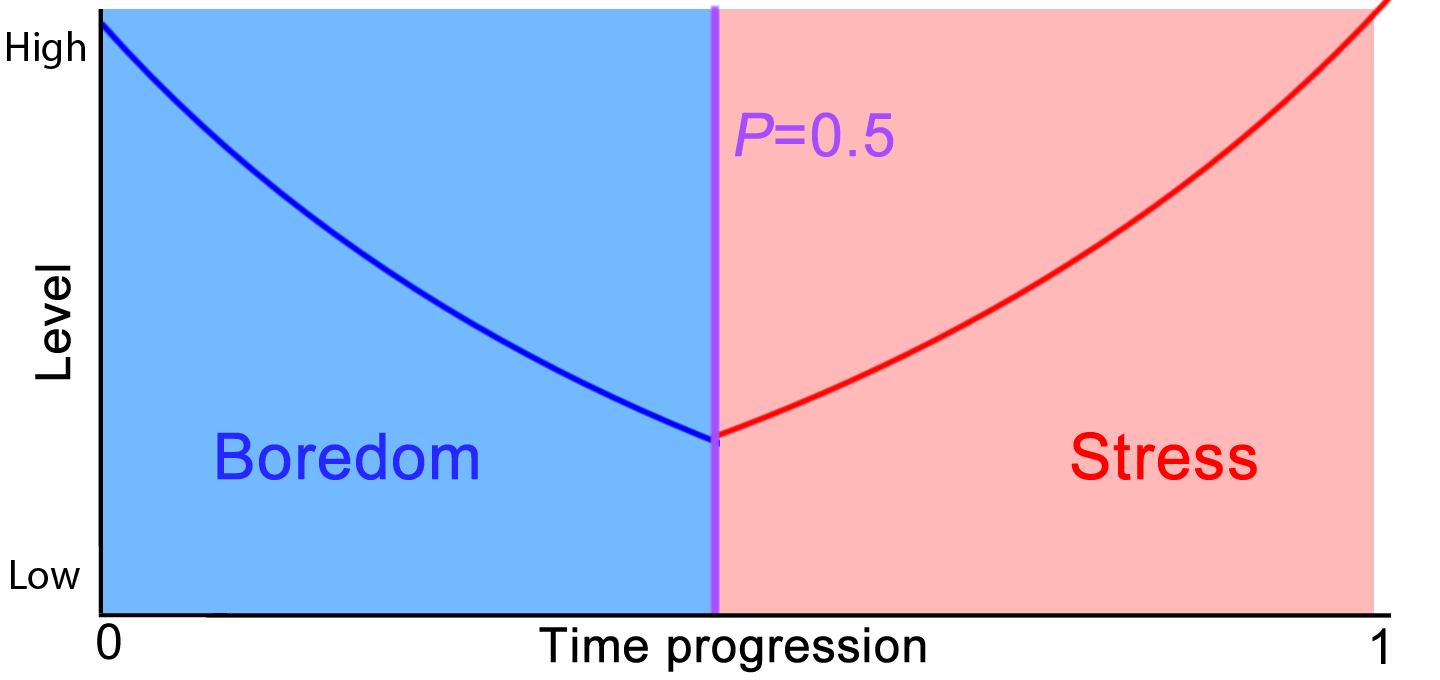
\includegraphics[width=0.8\textwidth]{figures/machine-learning-labeling-approach-A.png}
%    \caption{Labeling approach for the training of the user-tailored model based on a fixed point of division $P$ for both boredom and stress samples.}
%    \label{fig:machine-learning-labeling-approach-A}
%\end{figure}

%The video recordings that will be used in the tasks are related to experiment 1, whose games were designed to work as calibration games. As previously described in section \ref{sec:contributions}, those calibration games feature a progression from a boring to a stressful state. That configuration will be used as the foundation for the labeling process of emotional states during the training of the model, as well as ground truth for its testing.

%\begin{figure}[h]
%    \centering
%    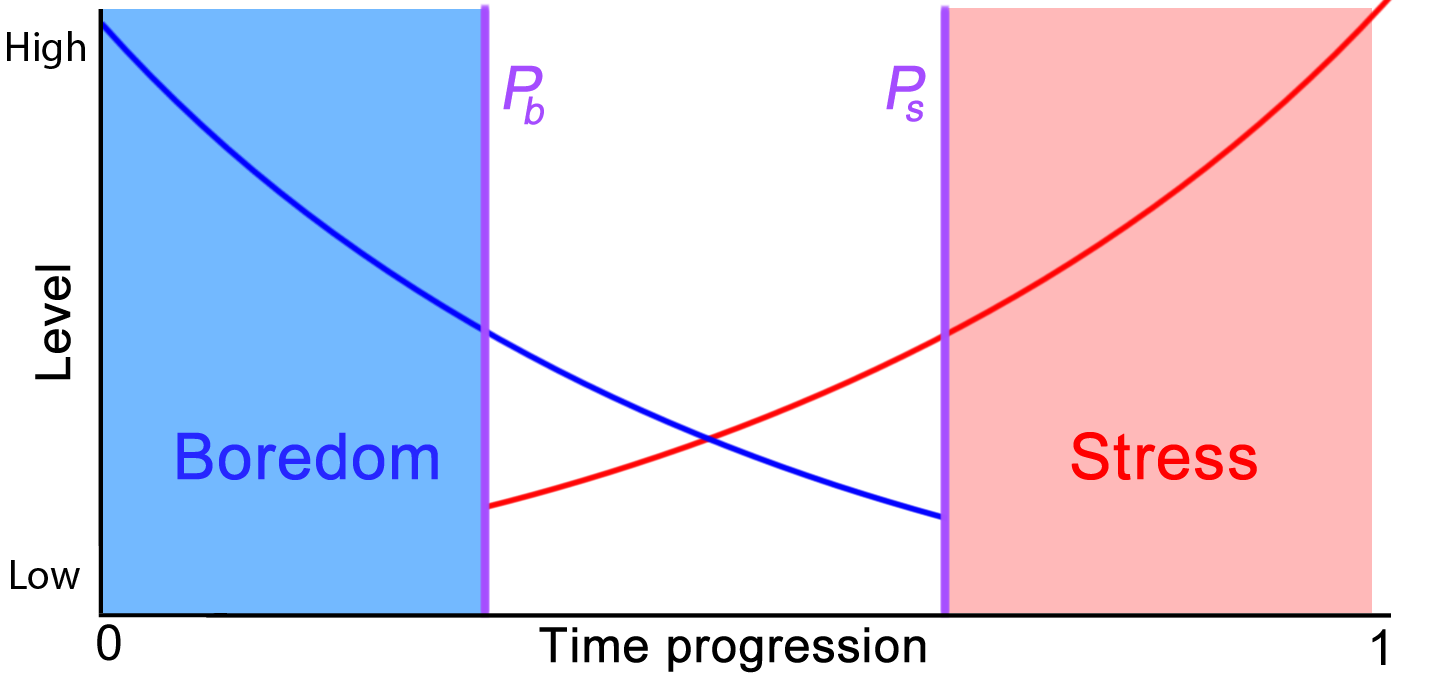
\includegraphics[width=0.8\textwidth]{figures/machine-learning-labeling-approach-B.png}
%    \caption{Labeling approach for the training of the user-tailored model based on varying points of division: $P_b$ (boredom samples) and $P_s$ (stress samples).}
%    \label{fig:machine-learning-labeling-approach-B}
%\end{figure}

%The training of the emotion detection model will be conducted according to two different strategies. In both approaches, the two games used as training sets will have their user signals sampled at a fixed interval of $T$ seconds, being $T$ empirically defined. The labeling of a sample as boredom or stress, however, will be different.

%Approach \textbf{A}, illustrated in Figure \ref{fig:machine-learning-labeling-approach-A}, assumes that $P$ represents the time progression of each game, e.g. $P=0$ is the starting point of the game and $P=1$ is its end point. Each game will then be divided in two equal parts ($P=0.5$). Samples from the first half of the game will be labeled as boredom, while samples from the second half will be labeled as stress. The division is based on the assumption that the middle of the games accurately separates in time the self-reported perceptions of boredom and stress made by the subjects.

%Approach \textbf{B}, illustrated in Figure \ref{fig:machine-learning-labeling-approach-B}, has each game divided in two parts: boredom, i.e. $P_b$, and stress, i.e. $P_s$, whose size (duration in time) will be calculated based on the self-reported answers given by subjects regarding boredom and stress. Samples from the $P_s$ part will be labeled as stress, while the samples from the $P_b$ part will be labeled as boredom. Approach \textbf{B} tries to mitigate the assumption that the middle point of the games perfectly divides the perceptions of boredom and stress. The approach accounts for the informed levels of boredom and stress of the subject, labeling only the samples within the areas more likely to accurately reflect the self-reported emotional states.

%The testing process will be similar for both approaches \textbf{A} and \textbf{B}. Samples from the game used as a testing set will be collected at a fixed interval of $K$ seconds, which will be larger than $T$ and also defined empirically. The associated labeling of the samples will be based on their position according to the rules of division points, i.e. $P$, $P_b$ or $P_s$. Sample points that eventually are not labeled, e.g. middle points in approach \textbf{B}, will be labeled as neutral.

%Following the described procedure, after all machine learning techniques are tested, they will have several resulting accuracy scores. The technique with the highest mean for the accuracy score will be selected. The following machine learning and classification techniques will be initially used in the tests: Support Vector Machine (SVM) using a radial basis, C-Support Vector Classification (C-SVC) using a linear kernel, K-nearest neighbours (K-nn), AdaBoost using nearest mean classifiers, Naive Bayers, and neural networks probably represented by convolution networks (convnets). Previous work \parencite{samara2016sensing,akakin2010spatiotemporal} also suggest a process involving decision fusion or a hierarchy of two or more classifiers working on different feature sets to improve prediction rates. Those approaches will probably be investigated as well.

%\subsection{Challenges and unresolved issues}

%One of the main unresolved issues regarding the use of a machine learning model is regarding its input features. Computer vision will be used to remotely extract a set of signals from the users, e.g. HR and the position of facial landmarks, however how those signals will be packeged as inputs for the machine learning model is still undefined.

%The current idea is to use a direct and discrete approach where the set of extracted signals from each frame of the video being analyzed is used as is. This approach does not explicitly feed the model with information regarding the variations of the extracted signals, e.g. HR decreased 5 bpm in the last 10 seconds, instead current information from each frame is used as input, e.g. HR is 60 bpm now. The approach relies on the principle that the machine learning model will recognize any patterns regarding the variation of signals among the different samples over time, modeling those patterns as the desired mapping of emotional states.

%Another possible solution is to provide the model with the variations of the signals, which demands a pre-processing of the extracted signals before feeding them into the model. In such scenario, each extracted signal will be accompanied by additional data, e.g. standard deviation, mean, etc. Ideally the machine learning model will better account for the variations of the signals and the emotional states. If a convolutional neural network is used as a machine learning solution, for instance, each signal can be used as input to the model in the form of a matrix. In that case each row of the matrix contains a segment of the signal at different times and the convnet will automatically find a way to model such changes into emotional states.
